\documentclass[aspectratio=169,11pt]{beamer}
% =====================================================================
%  pds-beamer.tex — Estilo común de las transparencias.
%
%  Uso (desde teoría/Tx/transparencias/):
%     \documentclass[aspectratio=169,11pt]{beamer}
%     % =====================================================================
%  pds-beamer.tex — Estilo común de las transparencias.
%
%  Uso (desde teoría/Tx/transparencias/):
%     \documentclass[aspectratio=169,11pt]{beamer}
%     % =====================================================================
%  pds-beamer.tex — Estilo común de las transparencias.
%
%  Uso (desde teoría/Tx/transparencias/):
%     \documentclass[aspectratio=169,11pt]{beamer}
%     \input{../../comun/pds-beamer}
%     \title{...}  \subtitle{Tema x · ...}
%     \begin{document}
%       \portada
%       ...
%     \end{document}
%  Compilar con:  latexmk -xelatex  (o «make» desde teoría/)
% =====================================================================

\usetheme{Boadilla}
\usecolortheme{orchid}
\usefonttheme{professionalfonts}
\setbeamercovered{transparent}
\setbeamersize{text margin left=0.8cm, text margin right=0.8cm}
\setbeamertemplate{navigation symbols}{}
\setbeamertemplate{itemize item}[square]
\setbeamertemplate{itemize subitem}[circle]
\setbeamertemplate{itemize subsubitem}[triangle]
\setbeamertemplate{enumerate item}[square]
\setbeamertemplate{enumerate subitem}[circle]
\setbeamertemplate{caption}{\raggedright\insertcaption\par}

\input{../../comun/pds-comun.tex}

% Tipografía: Fira Sans + Fira Math (legibles en proyector)
\usepackage{fontspec}
\usepackage{unicode-math}
% Se cargan por nombre de fichero para que funcionen con cualquier
% instalación de TeX Live (o MiKTeX) sin instalar fuentes en el sistema.
\setmainfont{FiraSans}[Extension=.otf, UprightFont=*-Regular, BoldFont=*-SemiBold,
  ItalicFont=*-Italic, BoldItalicFont=*-SemiBoldItalic]
\setsansfont{FiraSans}[Extension=.otf, UprightFont=*-Regular, BoldFont=*-SemiBold,
  ItalicFont=*-Italic, BoldItalicFont=*-SemiBoldItalic]
\setmonofont{FiraMono}[Extension=.otf, UprightFont=*-Regular, BoldFont=*-Medium, AutoFakeSlant=0.15, Scale=0.92]
\setmathfont{FiraMath-Regular.otf}
\setmathfont{latinmodern-math.otf}[range={"229B,"22EE,"22F1}]

% Colores del tema ajustados a la paleta común (más contraste)
\setbeamercolor{structure}{fg=pdsazul}
\setbeamercolor{alerted text}{fg=pdsrojo}
\setbeamercolor{example text}{fg=pdsverde}
\setbeamercolor{block title}{bg=pdsazul, fg=white}
\setbeamercolor{block body}{bg=pdsfondo}
\setbeamercolor{block title alerted}{bg=pdsrojo, fg=white}
\setbeamercolor{block body alerted}{bg=pdsrojo!6}
\setbeamercolor{block title example}{bg=pdsverde, fg=white}
\setbeamercolor{block body example}{bg=pdsverde!6}
\setbeamercolor{frametitle}{fg=pdsazul, bg=white}
\setbeamerfont{frametitle}{size=\large, series=\bfseries}
\setbeamerfont{block title}{size=\normalsize, series=\bfseries}
\setbeamertemplate{blocks}[rounded][shadow=false]

% Logo en la esquina superior derecha de cada transparencia
\pgfdeclareimage[height=0.8cm]{logo}{../../comun/ucm.png}
\addtobeamertemplate{frametitle}{}{%
  \begin{tikzpicture}[remember picture, overlay]
    \node[anchor=north east, inner sep=0pt] at ([xshift=-0.25cm, yshift=-0.2cm]current page.north east) {\pgfuseimage{logo}};
  \end{tikzpicture}}

% Datos de portada
\author[\autorescorto]{\autores}
\institute[UCM]{\footnotesize\departamento\\\universidad}
\date[\curso]{\footnotesize\grado\\\curso}

\newcommand{\portada}{%
  \begin{frame}[plain]
    \begin{center}
      
\includegraphics[height=1.9cm]{../../comun/ucm.png}
    \end{center}
    \vspace{-0.4cm}
    \titlepage
  \end{frame}}

% Índice al empezar cada sección
\AtBeginSection[]{%
  \begin{frame}{Contenido}
    \tableofcontents[currentsection, hideothersubsections]
  \end{frame}}

\renewcommand{\pdscodesize}{\scriptsize}

% Utilidades
% \herramienta{T1-convolucion-continua}: enlace a la página publicada de
% herramientas/html (se abre en el navegador, sin instalar nada).
% \herramientaservidor{server/....py}: app que necesita Python (bokeh serve).
\newcommand{\urlherramientas}{https://ucm-237.github.io/PdS/}
\newcommand{\herramienta}[1]{%
  \par\vfill\hfill{\scriptsize\color{pdsgris}\faIcon\ \href{\urlherramientas#1.html}{Herramienta interactiva: \texttt{#1}}}}
\newcommand{\herramientaservidor}[1]{%
  \par\vfill\hfill{\scriptsize\color{pdsgris}\faIcon\ Herramienta interactiva (con Python): \texttt{herramientas/#1}}}
\newcommand{\faIcon}{\textbf{▶}}
\newcommand{\gris}[1]{{\color{pdsgris}#1}}
\newcommand{\nota}[1]{\par\vspace{2pt}{\footnotesize\color{pdsgris}\textit{#1}}\par}
% Nota sobre una errata de versiones anteriores (solo con \ERRATAS)
\newcommand{\errata}[1]{\iferratas\nota{Errata de versiones anteriores: #1}\fi}
\newcommand{\apuntes}[1]{\nota{Más detalle en los apuntes, #1.}}

% Bloques con nombre en castellano
\newenvironment{definicion}[1][Definición]{\begin{block}{#1}}{\end{block}}
\newenvironment{importante}[1][Importante]{\begin{alertblock}{#1}}{\end{alertblock}}
\newenvironment{ejemplo}[1][Ejemplo]{\begin{exampleblock}{#1}}{\end{exampleblock}}

%     \title{...}  \subtitle{Tema x · ...}
%     \begin{document}
%       \portada
%       ...
%     \end{document}
%  Compilar con:  latexmk -xelatex  (o «make» desde teoría/)
% =====================================================================

\usetheme{Boadilla}
\usecolortheme{orchid}
\usefonttheme{professionalfonts}
\setbeamercovered{transparent}
\setbeamersize{text margin left=0.8cm, text margin right=0.8cm}
\setbeamertemplate{navigation symbols}{}
\setbeamertemplate{itemize item}[square]
\setbeamertemplate{itemize subitem}[circle]
\setbeamertemplate{itemize subsubitem}[triangle]
\setbeamertemplate{enumerate item}[square]
\setbeamertemplate{enumerate subitem}[circle]
\setbeamertemplate{caption}{\raggedright\insertcaption\par}

% =====================================================================
%  pds-comun.tex — Paquetes, colores y estilos de código comunes a
%  transparencias, apuntes y hojas de ejercicios. Compilar con XeLaTeX.
%  No cargar directamente: lo cargan pds-beamer.tex y pds-apuntes.tex.
% =====================================================================

\usepackage{polyglossia}
\setmainlanguage{spanish}
\usepackage{mathtools}
\usepackage{graphicx}
\usepackage{booktabs}
\usepackage{multirow}
\usepackage{array}
\usepackage{xcolor}
\usepackage{tikz}
\usetikzlibrary{positioning,arrows.meta,calc,shapes.geometric,decorations.pathreplacing}
\usepackage{listings}
\usepackage{siunitx}
\sisetup{output-decimal-marker={,}, group-separator={\,}, per-mode=symbol}

% Notas de erratas de versiones anteriores: no se imprimen salvo que se
% defina \ERRATAS antes de cargar el estilo (make ERRATAS=1)
\newif\iferratas
\ifdefined\ERRATAS \erratastrue \fi

% Ruta común (logo y figuras compartidas)
\providecommand{\rutacomun}{../../comun/}
\input{\rutacomun datos.tex}

% ---------------------------------------------------------------------
%  Paleta (la misma que usan las figuras generadas con Python,
%  ver comun/pds_estilo.py)
% ---------------------------------------------------------------------
\definecolor{pdsazul}{HTML}{2B3A8C}
\definecolor{pdsrojo}{HTML}{C0392B}
\definecolor{pdsverde}{HTML}{1E7B4F}
\definecolor{pdsnaranja}{HTML}{D9822B}
\definecolor{pdsgris}{HTML}{5A5A66}
\definecolor{pdsfondo}{HTML}{F3F4FA}
\definecolor{pdscodigo}{HTML}{F7F7F2}

% ---------------------------------------------------------------------
%  Diagramas de bloques (TikZ)
% ---------------------------------------------------------------------
\tikzset{
  bloque/.style={rectangle, rounded corners=2pt, draw=pdsazul!80, fill=pdsfondo,
                 very thick, minimum height=8mm, minimum width=14mm, align=center},
  sumador/.style={circle, draw=pdsazul!80, fill=pdsfondo, thick, inner sep=1.5pt},
  flecha/.style={-{Stealth[length=2.2mm]}, thick, pdsgris},
}

% ---------------------------------------------------------------------
%  Código: Python y Matlab en paralelo
% ---------------------------------------------------------------------
\newcommand{\pdscodesize}{\footnotesize}
\lstdefinestyle{pds}{
  basicstyle=\ttfamily\pdscodesize,
  keywordstyle=\color{pdsazul}\bfseries,
  commentstyle=\color{pdsverde}\itshape,
  stringstyle=\color{pdsrojo},
  numbers=none,
  backgroundcolor=\color{pdscodigo},
  frame=single, rulecolor=\color{pdsgris!40}, framerule=0.4pt,
  xleftmargin=2pt, xrightmargin=2pt, aboveskip=2pt, belowskip=2pt,
  columns=fullflexible, keepspaces=true,
  showstringspaces=false, breaklines=true, tabsize=4,
  upquote=true,
  % Con XeLaTeX, listings desordena los caracteres no ASCII junto a
  % dígitos («2π» sale «π2»): se sustituyen por su versión matemática.
  literate={π}{{$\pi$}}1 {δ}{{$\delta$}}1 {ω}{{$\omega$}}1 {Ω}{{$\Omega$}}1
           {≈}{{$\approx$}}1 {µ}{{$\mu$}}1 {·}{{$\cdot$}}1 {α}{{$\alpha$}}1
           {á}{{á}}1 {é}{{é}}1 {í}{{í}}1 {ó}{{ó}}1 {ú}{{ú}}1 {ñ}{{ñ}}1 {¿}{{¿}}1,
}
\lstdefinestyle{python}{style=pds, language=Python,
  morekeywords={as,True,False,None}}
\lstdefinestyle{matlab}{style=pds, language=Matlab,
  morekeywords={function,end,true,false}}

% \codigo{<ruta sin extensión>} muestra el mismo ejemplo en Python
% y en Matlab, uno al lado del otro. Los ficheros viven en
% ../codigo/python/<nombre>.py y ../codigo/matlab/<nombre>.m y se
% ejecutan en las pruebas (make prueba-codigo).
\newcommand{\rutacodigo}{../codigo/}
\newcommand{\codigoetiqueta}[1]{{\sffamily\scriptsize\bfseries\color{pdsgris}#1}}
\newcommand{\codigo}[2][]{%
  \par\noindent
  \begin{minipage}[t]{0.495\linewidth}
    \codigoetiqueta{Python}\par\vspace{1pt}
    \lstinputlisting[style=python,#1]{\rutacodigo python/#2.py}
  \end{minipage}\hfill
  \begin{minipage}[t]{0.495\linewidth}
    \codigoetiqueta{Matlab}\par\vspace{1pt}
    \lstinputlisting[style=matlab,#1]{\rutacodigo matlab/#2.m}
  \end{minipage}\par}

\input{\rutacomun notacion.tex}


% Tipografía: Fira Sans + Fira Math (legibles en proyector)
\usepackage{fontspec}
\usepackage{unicode-math}
% Se cargan por nombre de fichero para que funcionen con cualquier
% instalación de TeX Live (o MiKTeX) sin instalar fuentes en el sistema.
\setmainfont{FiraSans}[Extension=.otf, UprightFont=*-Regular, BoldFont=*-SemiBold,
  ItalicFont=*-Italic, BoldItalicFont=*-SemiBoldItalic]
\setsansfont{FiraSans}[Extension=.otf, UprightFont=*-Regular, BoldFont=*-SemiBold,
  ItalicFont=*-Italic, BoldItalicFont=*-SemiBoldItalic]
\setmonofont{FiraMono}[Extension=.otf, UprightFont=*-Regular, BoldFont=*-Medium, AutoFakeSlant=0.15, Scale=0.92]
\setmathfont{FiraMath-Regular.otf}
\setmathfont{latinmodern-math.otf}[range={"229B,"22EE,"22F1}]

% Colores del tema ajustados a la paleta común (más contraste)
\setbeamercolor{structure}{fg=pdsazul}
\setbeamercolor{alerted text}{fg=pdsrojo}
\setbeamercolor{example text}{fg=pdsverde}
\setbeamercolor{block title}{bg=pdsazul, fg=white}
\setbeamercolor{block body}{bg=pdsfondo}
\setbeamercolor{block title alerted}{bg=pdsrojo, fg=white}
\setbeamercolor{block body alerted}{bg=pdsrojo!6}
\setbeamercolor{block title example}{bg=pdsverde, fg=white}
\setbeamercolor{block body example}{bg=pdsverde!6}
\setbeamercolor{frametitle}{fg=pdsazul, bg=white}
\setbeamerfont{frametitle}{size=\large, series=\bfseries}
\setbeamerfont{block title}{size=\normalsize, series=\bfseries}
\setbeamertemplate{blocks}[rounded][shadow=false]

% Logo en la esquina superior derecha de cada transparencia
\pgfdeclareimage[height=0.8cm]{logo}{../../comun/ucm.png}
\addtobeamertemplate{frametitle}{}{%
  \begin{tikzpicture}[remember picture, overlay]
    \node[anchor=north east, inner sep=0pt] at ([xshift=-0.25cm, yshift=-0.2cm]current page.north east) {\pgfuseimage{logo}};
  \end{tikzpicture}}

% Datos de portada
\author[\autorescorto]{\autores}
\institute[UCM]{\footnotesize\departamento\\\universidad}
\date[\curso]{\footnotesize\grado\\\curso}

\newcommand{\portada}{%
  \begin{frame}[plain]
    \begin{center}
      
\includegraphics[height=1.9cm]{../../comun/ucm.png}
    \end{center}
    \vspace{-0.4cm}
    \titlepage
  \end{frame}}

% Índice al empezar cada sección
\AtBeginSection[]{%
  \begin{frame}{Contenido}
    \tableofcontents[currentsection, hideothersubsections]
  \end{frame}}

\renewcommand{\pdscodesize}{\scriptsize}

% Utilidades
% \herramienta{T1-convolucion-continua}: enlace a la página publicada de
% herramientas/html (se abre en el navegador, sin instalar nada).
% \herramientaservidor{server/....py}: app que necesita Python (bokeh serve).
\newcommand{\urlherramientas}{https://ucm-237.github.io/PdS/}
\newcommand{\herramienta}[1]{%
  \par\vfill\hfill{\scriptsize\color{pdsgris}\faIcon\ \href{\urlherramientas#1.html}{Herramienta interactiva: \texttt{#1}}}}
\newcommand{\herramientaservidor}[1]{%
  \par\vfill\hfill{\scriptsize\color{pdsgris}\faIcon\ Herramienta interactiva (con Python): \texttt{herramientas/#1}}}
\newcommand{\faIcon}{\textbf{▶}}
\newcommand{\gris}[1]{{\color{pdsgris}#1}}
\newcommand{\nota}[1]{\par\vspace{2pt}{\footnotesize\color{pdsgris}\textit{#1}}\par}
% Nota sobre una errata de versiones anteriores (solo con \ERRATAS)
\newcommand{\errata}[1]{\iferratas\nota{Errata de versiones anteriores: #1}\fi}
\newcommand{\apuntes}[1]{\nota{Más detalle en los apuntes, #1.}}

% Bloques con nombre en castellano
\newenvironment{definicion}[1][Definición]{\begin{block}{#1}}{\end{block}}
\newenvironment{importante}[1][Importante]{\begin{alertblock}{#1}}{\end{alertblock}}
\newenvironment{ejemplo}[1][Ejemplo]{\begin{exampleblock}{#1}}{\end{exampleblock}}

%     \title{...}  \subtitle{Tema x · ...}
%     \begin{document}
%       \portada
%       ...
%     \end{document}
%  Compilar con:  latexmk -xelatex  (o «make» desde teoría/)
% =====================================================================

\usetheme{Boadilla}
\usecolortheme{orchid}
\usefonttheme{professionalfonts}
\setbeamercovered{transparent}
\setbeamersize{text margin left=0.8cm, text margin right=0.8cm}
\setbeamertemplate{navigation symbols}{}
\setbeamertemplate{itemize item}[square]
\setbeamertemplate{itemize subitem}[circle]
\setbeamertemplate{itemize subsubitem}[triangle]
\setbeamertemplate{enumerate item}[square]
\setbeamertemplate{enumerate subitem}[circle]
\setbeamertemplate{caption}{\raggedright\insertcaption\par}

% =====================================================================
%  pds-comun.tex — Paquetes, colores y estilos de código comunes a
%  transparencias, apuntes y hojas de ejercicios. Compilar con XeLaTeX.
%  No cargar directamente: lo cargan pds-beamer.tex y pds-apuntes.tex.
% =====================================================================

\usepackage{polyglossia}
\setmainlanguage{spanish}
\usepackage{mathtools}
\usepackage{graphicx}
\usepackage{booktabs}
\usepackage{multirow}
\usepackage{array}
\usepackage{xcolor}
\usepackage{tikz}
\usetikzlibrary{positioning,arrows.meta,calc,shapes.geometric,decorations.pathreplacing}
\usepackage{listings}
\usepackage{siunitx}
\sisetup{output-decimal-marker={,}, group-separator={\,}, per-mode=symbol}

% Notas de erratas de versiones anteriores: no se imprimen salvo que se
% defina \ERRATAS antes de cargar el estilo (make ERRATAS=1)
\newif\iferratas
\ifdefined\ERRATAS \erratastrue \fi

% Ruta común (logo y figuras compartidas)
\providecommand{\rutacomun}{../../comun/}
\input{\rutacomun datos.tex}

% ---------------------------------------------------------------------
%  Paleta (la misma que usan las figuras generadas con Python,
%  ver comun/pds_estilo.py)
% ---------------------------------------------------------------------
\definecolor{pdsazul}{HTML}{2B3A8C}
\definecolor{pdsrojo}{HTML}{C0392B}
\definecolor{pdsverde}{HTML}{1E7B4F}
\definecolor{pdsnaranja}{HTML}{D9822B}
\definecolor{pdsgris}{HTML}{5A5A66}
\definecolor{pdsfondo}{HTML}{F3F4FA}
\definecolor{pdscodigo}{HTML}{F7F7F2}

% ---------------------------------------------------------------------
%  Diagramas de bloques (TikZ)
% ---------------------------------------------------------------------
\tikzset{
  bloque/.style={rectangle, rounded corners=2pt, draw=pdsazul!80, fill=pdsfondo,
                 very thick, minimum height=8mm, minimum width=14mm, align=center},
  sumador/.style={circle, draw=pdsazul!80, fill=pdsfondo, thick, inner sep=1.5pt},
  flecha/.style={-{Stealth[length=2.2mm]}, thick, pdsgris},
}

% ---------------------------------------------------------------------
%  Código: Python y Matlab en paralelo
% ---------------------------------------------------------------------
\newcommand{\pdscodesize}{\footnotesize}
\lstdefinestyle{pds}{
  basicstyle=\ttfamily\pdscodesize,
  keywordstyle=\color{pdsazul}\bfseries,
  commentstyle=\color{pdsverde}\itshape,
  stringstyle=\color{pdsrojo},
  numbers=none,
  backgroundcolor=\color{pdscodigo},
  frame=single, rulecolor=\color{pdsgris!40}, framerule=0.4pt,
  xleftmargin=2pt, xrightmargin=2pt, aboveskip=2pt, belowskip=2pt,
  columns=fullflexible, keepspaces=true,
  showstringspaces=false, breaklines=true, tabsize=4,
  upquote=true,
  % Con XeLaTeX, listings desordena los caracteres no ASCII junto a
  % dígitos («2π» sale «π2»): se sustituyen por su versión matemática.
  literate={π}{{$\pi$}}1 {δ}{{$\delta$}}1 {ω}{{$\omega$}}1 {Ω}{{$\Omega$}}1
           {≈}{{$\approx$}}1 {µ}{{$\mu$}}1 {·}{{$\cdot$}}1 {α}{{$\alpha$}}1
           {á}{{á}}1 {é}{{é}}1 {í}{{í}}1 {ó}{{ó}}1 {ú}{{ú}}1 {ñ}{{ñ}}1 {¿}{{¿}}1,
}
\lstdefinestyle{python}{style=pds, language=Python,
  morekeywords={as,True,False,None}}
\lstdefinestyle{matlab}{style=pds, language=Matlab,
  morekeywords={function,end,true,false}}

% \codigo{<ruta sin extensión>} muestra el mismo ejemplo en Python
% y en Matlab, uno al lado del otro. Los ficheros viven en
% ../codigo/python/<nombre>.py y ../codigo/matlab/<nombre>.m y se
% ejecutan en las pruebas (make prueba-codigo).
\newcommand{\rutacodigo}{../codigo/}
\newcommand{\codigoetiqueta}[1]{{\sffamily\scriptsize\bfseries\color{pdsgris}#1}}
\newcommand{\codigo}[2][]{%
  \par\noindent
  \begin{minipage}[t]{0.495\linewidth}
    \codigoetiqueta{Python}\par\vspace{1pt}
    \lstinputlisting[style=python,#1]{\rutacodigo python/#2.py}
  \end{minipage}\hfill
  \begin{minipage}[t]{0.495\linewidth}
    \codigoetiqueta{Matlab}\par\vspace{1pt}
    \lstinputlisting[style=matlab,#1]{\rutacodigo matlab/#2.m}
  \end{minipage}\par}

\input{\rutacomun notacion.tex}


% Tipografía: Fira Sans + Fira Math (legibles en proyector)
\usepackage{fontspec}
\usepackage{unicode-math}
% Se cargan por nombre de fichero para que funcionen con cualquier
% instalación de TeX Live (o MiKTeX) sin instalar fuentes en el sistema.
\setmainfont{FiraSans}[Extension=.otf, UprightFont=*-Regular, BoldFont=*-SemiBold,
  ItalicFont=*-Italic, BoldItalicFont=*-SemiBoldItalic]
\setsansfont{FiraSans}[Extension=.otf, UprightFont=*-Regular, BoldFont=*-SemiBold,
  ItalicFont=*-Italic, BoldItalicFont=*-SemiBoldItalic]
\setmonofont{FiraMono}[Extension=.otf, UprightFont=*-Regular, BoldFont=*-Medium, AutoFakeSlant=0.15, Scale=0.92]
\setmathfont{FiraMath-Regular.otf}
\setmathfont{latinmodern-math.otf}[range={"229B,"22EE,"22F1}]

% Colores del tema ajustados a la paleta común (más contraste)
\setbeamercolor{structure}{fg=pdsazul}
\setbeamercolor{alerted text}{fg=pdsrojo}
\setbeamercolor{example text}{fg=pdsverde}
\setbeamercolor{block title}{bg=pdsazul, fg=white}
\setbeamercolor{block body}{bg=pdsfondo}
\setbeamercolor{block title alerted}{bg=pdsrojo, fg=white}
\setbeamercolor{block body alerted}{bg=pdsrojo!6}
\setbeamercolor{block title example}{bg=pdsverde, fg=white}
\setbeamercolor{block body example}{bg=pdsverde!6}
\setbeamercolor{frametitle}{fg=pdsazul, bg=white}
\setbeamerfont{frametitle}{size=\large, series=\bfseries}
\setbeamerfont{block title}{size=\normalsize, series=\bfseries}
\setbeamertemplate{blocks}[rounded][shadow=false]

% Logo en la esquina superior derecha de cada transparencia
\pgfdeclareimage[height=0.8cm]{logo}{../../comun/ucm.png}
\addtobeamertemplate{frametitle}{}{%
  \begin{tikzpicture}[remember picture, overlay]
    \node[anchor=north east, inner sep=0pt] at ([xshift=-0.25cm, yshift=-0.2cm]current page.north east) {\pgfuseimage{logo}};
  \end{tikzpicture}}

% Datos de portada
\author[\autorescorto]{\autores}
\institute[UCM]{\footnotesize\departamento\\\universidad}
\date[\curso]{\footnotesize\grado\\\curso}

\newcommand{\portada}{%
  \begin{frame}[plain]
    \begin{center}
      
\includegraphics[height=1.9cm]{../../comun/ucm.png}
    \end{center}
    \vspace{-0.4cm}
    \titlepage
  \end{frame}}

% Índice al empezar cada sección
\AtBeginSection[]{%
  \begin{frame}{Contenido}
    \tableofcontents[currentsection, hideothersubsections]
  \end{frame}}

\renewcommand{\pdscodesize}{\scriptsize}

% Utilidades
% \herramienta{T1-convolucion-continua}: enlace a la página publicada de
% herramientas/html (se abre en el navegador, sin instalar nada).
% \herramientaservidor{server/....py}: app que necesita Python (bokeh serve).
\newcommand{\urlherramientas}{https://ucm-237.github.io/PdS/}
\newcommand{\herramienta}[1]{%
  \par\vfill\hfill{\scriptsize\color{pdsgris}\faIcon\ \href{\urlherramientas#1.html}{Herramienta interactiva: \texttt{#1}}}}
\newcommand{\herramientaservidor}[1]{%
  \par\vfill\hfill{\scriptsize\color{pdsgris}\faIcon\ Herramienta interactiva (con Python): \texttt{herramientas/#1}}}
\newcommand{\faIcon}{\textbf{▶}}
\newcommand{\gris}[1]{{\color{pdsgris}#1}}
\newcommand{\nota}[1]{\par\vspace{2pt}{\footnotesize\color{pdsgris}\textit{#1}}\par}
% Nota sobre una errata de versiones anteriores (solo con \ERRATAS)
\newcommand{\errata}[1]{\iferratas\nota{Errata de versiones anteriores: #1}\fi}
\newcommand{\apuntes}[1]{\nota{Más detalle en los apuntes, #1.}}

% Bloques con nombre en castellano
\newenvironment{definicion}[1][Definición]{\begin{block}{#1}}{\end{block}}
\newenvironment{importante}[1][Importante]{\begin{alertblock}{#1}}{\end{alertblock}}
\newenvironment{ejemplo}[1][Ejemplo]{\begin{exampleblock}{#1}}{\end{exampleblock}}

\graphicspath{{../figuras/}}

\title[T6 · Variables aleatorias]{Señales aleatorias}
\subtitle{Tema 6 · Parte 1: variables aleatorias, muestreo y análisis}

\begin{document}
\portada

\begin{frame}{Objetivos del tema}
  \begin{itemize}
    \item Describir lo que no se puede predecir: ruido, interferencias, mensajes, medidas.
    \item \alert{Variables aleatorias}: funciones de probabilidad, media y varianza; generar muestras con el ordenador y estimar a partir de ellas.
    \item \alert{Varias variables}: distribución conjunta, independencia, covarianza y correlación.
    \item \alert{Señales aleatorias}: estacionariedad, ergodicidad, autocorrelación y correlación cruzada.
    \item \alert{Análisis espectral}: densidad espectral de potencia y respuesta de un sistema LTI a una señal aleatoria.
  \end{itemize}
  \bigskip
  \gris{Partes: 1 Variables aleatorias · 2 Varias variables · 3 Señales aleatorias · 4 Análisis espectral.}
\end{frame}

% =====================================================================
\section{Señales deterministas y aleatorias}

\begin{frame}{¿Por qué señales aleatorias?}
  \begin{center}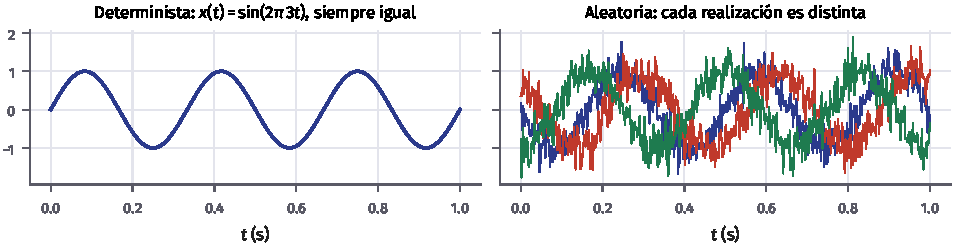
\includegraphics[width=0.95\linewidth]{deterministas_aleatorias}\end{center}
  \small
  \begin{itemize}
    \item Una señal \alert{determinista} se conoce exactamente en todo instante: una fórmula, una tabla.
    \item Una señal \alert{aleatoria} (o estocástica) no se puede predecir: cada vez que se observa sale distinta. Ruido térmico, voz, datos transmitidos, vibraciones, medidas de un sensor.
    \item No se describe valor a valor, sino \alert{estadísticamente}: qué valores son probables, cuánto varían, cómo se parecen los valores próximos.
  \end{itemize}
\end{frame}

% =====================================================================
\section{Variable aleatoria}

\begin{frame}{Variable aleatoria}
  \begin{definicion}[Variable aleatoria]
    Una \alert{variable aleatoria} $X$ asigna un número a cada resultado de un experimento aleatorio. Antes del experimento solo se sabe con qué probabilidad tomará cada valor; el valor obtenido, $x$, es una \alert{realización} o muestra.
  \end{definicion}
  \small
  \begin{itemize}
    \item \alert{Discreta}: toma valores sueltos $x_i$ (la cara de un dado, un bit recibido). Se describe con la \alert{función de probabilidad} $p_X(x_i)=P(X=x_i)$, con $\sum_ip_X(x_i)=1$.
    \item \alert{Continua}: toma valores en un intervalo (una tensión de ruido). Se describe con la \alert{función de densidad} $f_X(x)\ge0$:
    \[
      P(a<X\le b)=\int_a^bf_X(x)\dd x,\qquad\int_{-\infty}^{\infty}f_X(x)\dd x=1 .
    \]
    $f_X(x)$ no es una probabilidad: puede ser mayor que 1, y $P(X=x)=0$.
  \end{itemize}
\end{frame}

\begin{frame}{Función de distribución}
  \begin{columns}[c]
    \begin{column}{0.4\textwidth}
      \small
      \[
        F_X(x)=P(X\le x)
      \]
      \begin{itemize}
        \item Vale para discretas y continuas.
        \item Crece de $F_X(-\infty)=0$ a $F_X(\infty)=1$.
        \item $P(a<X\le b)=F_X(b)-F_X(a)$.
        \item Continuas: $f_X(x)=\dv{F_X}{x}$.
        \item Discretas: escalones de altura $p_X(x_i)$ en cada $x_i$.
      \end{itemize}
    \end{column}
    \begin{column}{0.58\textwidth}
      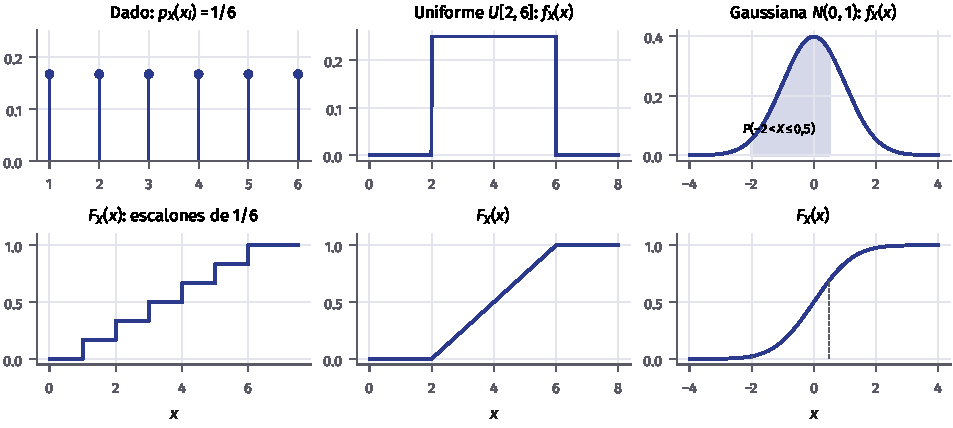
\includegraphics[width=\linewidth]{pmf_pdf_cdf}
    \end{column}
  \end{columns}
\end{frame}

\begin{frame}{Esperanza, media y varianza}
  \small
  \begin{definicion}[Esperanza]
    \[
      E\{g(X)\}=\sum_ig(x_i)\,p_X(x_i)\qquad\text{o}\qquad E\{g(X)\}=\int_{-\infty}^{\infty}g(x)\,f_X(x)\dd x
    \]
  \end{definicion}
  \begin{itemize}
    \item \alert{Media}: $\mu_X=E\{X\}$, el centro de gravedad de la distribución.
    \item \alert{Valor cuadrático medio}: $E\{X^2\}$. Si $X$ es una tensión sobre 1\,$\Omega$, es la potencia media.
    \item \alert{Varianza}: $\sigma_X^2=E\{(X-\mu_X)^2\}=E\{X^2\}-\mu_X^2$. Su raíz, $\sigma_X$, es la \alert{desviación típica}.
    \item La esperanza es lineal: $E\{aX+b\}=a\mu_X+b$ y $\operatorname{Var}\{aX+b\}=a^2\sigma_X^2$.
  \end{itemize}
  \begin{ejemplo}[Dado]
    $\mu_X=\frac{1+\dots+6}6=3{,}5$; $E\{X^2\}=\frac{91}6$; $\sigma_X^2=\frac{91}6-3{,}5^2=\frac{35}{12}$.
  \end{ejemplo}
\end{frame}

% =====================================================================
\section{Distribuciones habituales}

\begin{frame}{Uniforme y gaussiana}
  \begin{columns}[c]
    \begin{column}{0.5\textwidth}
      \small
      \alert{Uniforme} $\mathcal U[a,b]$:
      \[
        f_X(x)=\begin{cases}\frac1{b-a},&a\le x\le b\\0,&\text{resto}\end{cases}
      \]
      $\mu_X=\frac{a+b}2$, $\sigma_X^2=\frac{(b-a)^2}{12}$, $E\{X^2\}=\frac{a^2+ab+b^2}3$.
      \nota{Error de cuantificación, fase de una portadora, números aleatorios del ordenador.}
      \medskip
      \alert{Gaussiana} o normal $\mathcal N(\mu,\sigma^2)$:
      \[
        f_X(x)=\frac1{\sqrt{2\pi}\,\sigma}\,\e^{-\frac{(x-\mu)^2}{2\sigma^2}}
      \]
      \nota{Ruido térmico y, en general, la suma de muchas causas pequeñas e independientes (parte~2).}
    \end{column}
    \begin{column}{0.48\textwidth}
      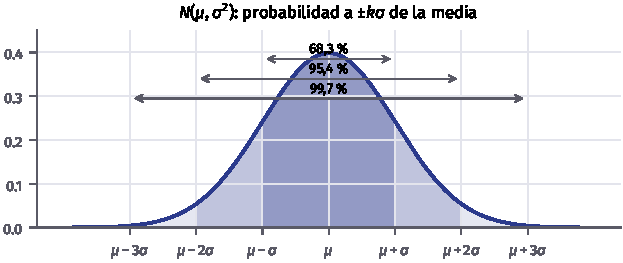
\includegraphics[width=\linewidth]{gaussiana}
      \small
      \begin{itemize}
        \item $Z=(X-\mu)/\sigma$ es $\mathcal N(0,1)$; $F_Z$ se tabula como $\Phi(z)$.
        \item $aX+b$ es $\mathcal N(a\mu+b,\,a^2\sigma^2)$.
      \end{itemize}
    \end{column}
  \end{columns}
\end{frame}

% =====================================================================
\section{Muestreo de variables aleatorias}

\begin{frame}{Generar muestras con el ordenador}
  \small
  \begin{itemize}
    \item Los generadores de números pseudoaleatorios dan muestras de $\mathcal U[0,1)$: \texttt{rand} en Matlab, \texttt{rng.random} en Python. A partir de ellas se obtiene cualquier distribución.
    \item \alert{Simular} un sistema con entradas aleatorias muchas veces permite estimar lo que es difícil de calcular: es el método de \alert{Monte Carlo}.
    \item Métodos:
    \begin{itemize}
      \item variables discretas: método de la ruleta;
      \item inversa de la función de distribución;
      \item Box-Muller para gaussianas (Matlab y Python traen \texttt{randn} y \texttt{rng.standard\_normal});
      \item aceptación y rechazo, cuando no se puede invertir $F_X$;
      \item mezclas.
    \end{itemize}
  \end{itemize}
  \nota{Fijar la semilla (\texttt{rng(0)} en Matlab, \texttt{np.random.default\_rng(0)} en Python) hace los resultados reproducibles.}
\end{frame}

\begin{frame}{Variables discretas: método de la ruleta}
  \begin{columns}[c]
    \begin{column}{0.5\textwidth}
      \small
      \begin{itemize}
        \item Se reparte $[0,1)$ en tramos de longitud $p_X(x_i)$, como los sectores de una ruleta.
        \item Se genera $u\sim\mathcal U[0,1)$ y se devuelve el $x_i$ cuyo tramo contiene a $u$:
        \[
          x=x_i\quad\text{si}\quad F_X(x_{i-1})\le u<F_X(x_i).
        \]
        \item El tramo $i$ mide $p_X(x_i)$, así que sale con esa probabilidad.
      \end{itemize}
    \end{column}
    \begin{column}{0.48\textwidth}
      \begin{ejemplo}[Dado cargado]
        \footnotesize
        $p=(0{,}1;\,0{,}1;\,0{,}1;\,0{,}1;\,0{,}1;\,0{,}5)$, $F=(0{,}1;\,0{,}2;\,\dots;\,0{,}5;\,1)$. Con $u=0{,}37$: $F(3)=0{,}3\le0{,}37<0{,}4=F(4)$, sale un 4. Con $u=0{,}62$ sale un 6.
      \end{ejemplo}
    \end{column}
  \end{columns}
  \errata{la condición de la ruleta debe incluir la igualdad en un extremo; si no, los $u$ que caen justo en un borde no tienen valor asignado.}
\end{frame}

\begin{frame}{En código: método de la ruleta}
  \codigo{ruleta}
\end{frame}

\begin{frame}{Inversa de la función de distribución}
  \begin{columns}[c]
    \begin{column}{0.4\textwidth}
      \small
      \begin{importante}[Resultado]
        Si $U\sim\mathcal U[0,1]$ y $F_X$ es continua y creciente, $X=F_X^{-1}(U)$ tiene distribución $F_X$.
      \end{importante}
      Porque $P(X\le x)=P(U\le F_X(x))=F_X(x)$.
      \medskip

      Exponencial: $F_X(x)=1-\e^{-\lambda x}$, así que
      \[
        x=-\frac1\lambda\ln(1-u).
      \]
    \end{column}
    \begin{column}{0.58\textwidth}
      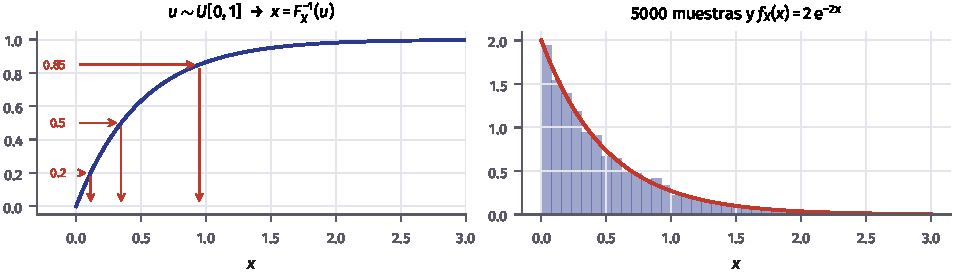
\includegraphics[width=\linewidth]{metodo_inversa}
      \nota{El método de la ruleta es la versión discreta de este. Aplicado al revés, $F_X(X)$ es uniforme: es la ecualización del histograma (tema~5).}
    \end{column}
  \end{columns}
\end{frame}

\begin{frame}{En código: exponencial e inversa}
  \codigo{muestreo_inversa}
  \nota{\texttt{var} de Matlab y \texttt{var(ddof=1)} de numpy dividen por $N-1$; \texttt{np.var} sin más, por $N$.}
\end{frame}

\begin{frame}{Gaussianas: Box-Muller}
  \begin{columns}[c]
    \begin{column}{0.52\textwidth}
      \small
      \begin{itemize}
        \item $F$ de la gaussiana no tiene inversa explícita.
        \item Truco: un par $(Z_1,Z_2)$ de gaussianas independientes, en polares, tiene ángulo uniforme y radio con $F_R(r)=1-\e^{-r^2/2}$, que sí se invierte.
        \item Con $u_1,u_2\sim\mathcal U[0,1)$ independientes:
        \[
          r=\sqrt{-2\ln(1-u_1)},\qquad\theta=2\pi u_2,
        \]
        \[
          z_1=r\cos\theta,\qquad z_2=r\sin\theta .
        \]
        \item Se obtiene un \alert{par} de muestras $\mathcal N(0,1)$ independientes. Para $\mathcal N(\mu,\sigma^2)$: $x=\mu+\sigma z$.
      \end{itemize}
    \end{column}
    \begin{column}{0.46\textwidth}
      \begin{ejemplo}[Una pareja]
        \footnotesize
        $u_1=0{,}6$, $u_2=0{,}1$: $r=\sqrt{-2\ln0{,}4}=1{,}354$, $\theta=0{,}2\pi$; $z_1=1{,}095$ y $z_2=0{,}796$.
      \end{ejemplo}
      \nota{La versión antigua decía «se genera un par…» sin terminar la frase.}
    \end{column}
  \end{columns}
\end{frame}

\begin{frame}{En código: Box-Muller}
  \codigo{box_muller}
\end{frame}

\begin{frame}{Aceptación y rechazo}
  \begin{columns}[c]
    \begin{column}{0.42\textwidth}
      \small
      \begin{itemize}
        \item Se busca una densidad $q(x)$ fácil de muestrear y un $M$ con
        \[
          Mq(x)\ge f(x)\quad\text{para todo }x .
        \]
        \item Se genera $x\sim q$ y $u\sim\mathcal U[0,1)$; se \alert{acepta} $x$ si $u\,Mq(x)\le f(x)$.
        \item Los puntos $(x,uMq(x))$ caen uniformes bajo $Mq$; los aceptados, uniformes bajo $f$.
        \item Se acepta una fracción $1/M$: conviene $Mq$ ajustada a $f$.
      \end{itemize}
    \end{column}
    \begin{column}{0.56\textwidth}
      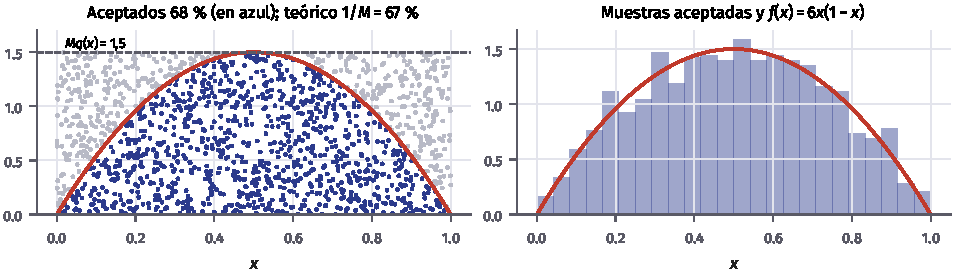
\includegraphics[width=\linewidth]{rechazo}
      \errata{la condición es $Mq(x)\ge f(x)$, con igualdad permitida, y no $Mq(x)-f(x)>0$.}
    \end{column}
  \end{columns}
\end{frame}

\begin{frame}{Mezclas}
  \begin{columns}[c]
    \begin{column}{0.42\textwidth}
      \small
      \[
        f_X(x)=\sum_{k=1}^K\pi_k\,f_k(x),\qquad\sum_k\pi_k=1
      \]
      \begin{itemize}
        \item Modela poblaciones con varios grupos (dos tipos de pieza, ruido con dos regímenes).
        \item Muestreo en dos pasos: elegir la componente $k$ con probabilidad $\pi_k$ (ruleta) y muestrear $f_k$.
      \end{itemize}
    \end{column}
    \begin{column}{0.56\textwidth}
      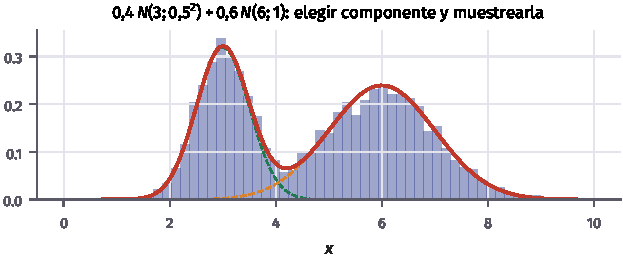
\includegraphics[width=\linewidth]{mezcla}
      \nota{La transparencia antigua dejaba la mezcla sin terminar: «$p_X(x)=0{,}4\mathcal N(x,3,0{,}5)+$».}
    \end{column}
  \end{columns}
\end{frame}

% =====================================================================
\section{Análisis de muestras}

\begin{frame}{Histograma}
  \begin{center}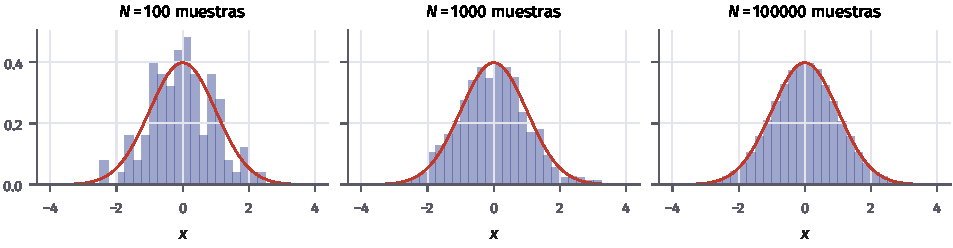
\includegraphics[width=0.95\linewidth]{histograma_n}\end{center}
  \small
  \begin{itemize}
    \item Se divide el eje en intervalos de anchura $\Delta$ y se cuentan las muestras $n_j$ de cada uno.
    \item $\hat f_X(x)=\frac{n_j}{N\Delta}$ en el intervalo $j$ estima la densidad (el área total es 1). Más muestras, mejor estimación; intervalos más estrechos, más detalle pero más ruido.
  \end{itemize}
  \nota{Matlab: \texttt{histogram(x, 'Normalization', 'pdf')}; Python: \texttt{plt.hist(x, density=True)}.}
\end{frame}

\begin{frame}{Estimadores}
  \small
  Con $N$ muestras independientes $x_1,\dots,x_N$:
  \[
    \hat\mu=\frac1N\sum_{i=1}^Nx_i,\qquad\hat\sigma^2=\frac1{N-1}\sum_{i=1}^N(x_i-\hat\mu)^2,\qquad\widehat{E\{g(X)\}}=\frac1N\sum_{i=1}^Ng(x_i).
  \]
  \begin{itemize}
    \item Son también variables aleatorias. $\hat\mu$ es \alert{insesgado} ($E\{\hat\mu\}=\mu$) y su varianza es $\sigma^2/N$: el error típico baja como $1/\sqrt N$.
    \item Con $N-1$ el estimador de la varianza es insesgado; con $N$ (el de máxima verosimilitud para la gaussiana) se queda corto en un factor $(N-1)/N$.
    \item \alert{Monte Carlo}: $E\{g(X)\}=\int g(x)f_X(x)\dd x$ se aproxima por la media de $g$ sobre las muestras, aunque la integral no tenga solución cerrada.
  \end{itemize}
  \errata{la suma de Monte Carlo usaba el índice $n$ y escribía $x_i$, y el estimador de la varianza dividía por $N$ sin advertir el sesgo.}
\end{frame}

\begin{frame}{Monte Carlo}
  \begin{center}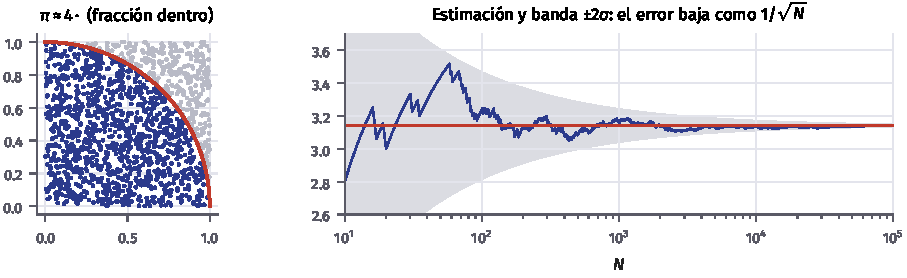
\includegraphics[width=0.72\linewidth]{montecarlo}\end{center}
  \codigo[basicstyle=\ttfamily\fontsize{6.3}{7.1}\selectfont]{montecarlo}
\end{frame}

% =====================================================================
\section*{Resumen}
\begin{frame}{Conceptos importantes}
  \begin{columns}[T]
    \begin{column}{0.5\textwidth}
      \begin{itemize}
        \item Variable aleatoria: discreta ($p_X$) o continua ($f_X$); $F_X(x)=P(X\le x)$.
        \item $E\{\cdot\}$ lineal; $\mu_X$, $E\{X^2\}$, $\sigma_X^2=E\{X^2\}-\mu_X^2$.
        \item Uniforme y gaussiana; $Z=(X-\mu)/\sigma$.
      \end{itemize}
    \end{column}
    \begin{column}{0.5\textwidth}
      \begin{itemize}
        \item Muestreo: ruleta, inversa, Box-Muller, rechazo, mezclas.
        \item Histograma normalizado $n_j/(N\Delta)$.
        \item Estimadores: media, varianza con $N-1$; error $\propto1/\sqrt N$.
      \end{itemize}
    \end{column}
  \end{columns}
  \bigskip
  \gris{Apuntes del Tema 6, sección 1 · Hoja de ejercicios, ejercicios 1–5.}
\end{frame}

\end{document}
